\chapter[The CMS experiment at LHC]{The CMS experiment at LHC}

The CMS experiment is one of the biggest particle physics experiments on the world. It is located at the ring of the LHC that is the main experience managed by CERN, the European Organization for Nuclear Research or Centre Europ\'{e}enne pour la Recherche Nucl\'{e}aire by its name on french. This center constitutes the biggest center for research on particle physics all over the world. All along its 60 years of existence, from 1954, 21 member states have been joining it, but an overall of 113 countries participate in different ways on this center. 

On the present chapter we discuss in detail different aspects of the LHC accelerator and the CMS experiment. In particular we make some emphasis in the CMS sub-detectors related to jets, objects that play the main role on the search that is the main subject of the present work. We also discuss the present state of both machines, their achievements and the challenges that were came through. Finally, also the expectations and goals for the upcoming run II are mentioned.  

\section{The Large Hadron Collider}
\label{sec:LHC}

The Large Hadron Collider, or LHC, is a machine that accelerates and collides protons and heavy ions. This machine is the biggest particle collider nowadays with a circumference of 27 km. It also achieves the greatest energy by a collider up to present, planned to be 14 TeV at the center of mass of the collision. On the first run of the machine only 8 TeV were achieved, and next run is planned to start with 13 TeV. It's located in French-Swiss border near to Geneva. The tunnel for the machine was carved around 100 m under the ground, 45 m under the Jura mountains and 170 m under the L\'{e}man lake with an inclination of around 1.4\%, sloping down towards the lake . This machine has used as much as possible old LEP buildings and sites, that was an electron-positron collider built between 1984 and 1989. 

The protons and heavy ions accelerated by the machine are collided in different points where dedicated experiments are located to detect and study the product from the collisions. The four main experiments located on the LHC ring are CMS, ATLAS, LHCb and ALICE. The first two are experiments of generic purpose where searches for new physics and also precision measurements are performed. LHCb is dedicated to the physics of the b-quark, and ALICE focuses on the study of the quark-gluon plasma produced from heavy ions collisions. However one of the principal objectives of the construction of the LHC was the discovery of the Higgs boson, generic searches on new physics have been conducted from the very beginning of the first data taking on 2009. Moreover, after the Higgs discovery on 2012 there is a growing effort on the searches for new physics and precision measurement on the properties of the Higgs.

The LHC is a complex machine composed of several parts. The two principal parts are the injector chain and the main ring. A diagram of the whole CERN complex can be seen in figure~\ref{fig:Complex}. The injector chain has different stages that pre-accelerate protons and heavy ions to be injected into the main ring of LHC. In the main ring the protons and heavy ions are fully accelerated and collided in four different points over the ring.

\begin{figure}[!Hhtbp]
  \begin{center}
    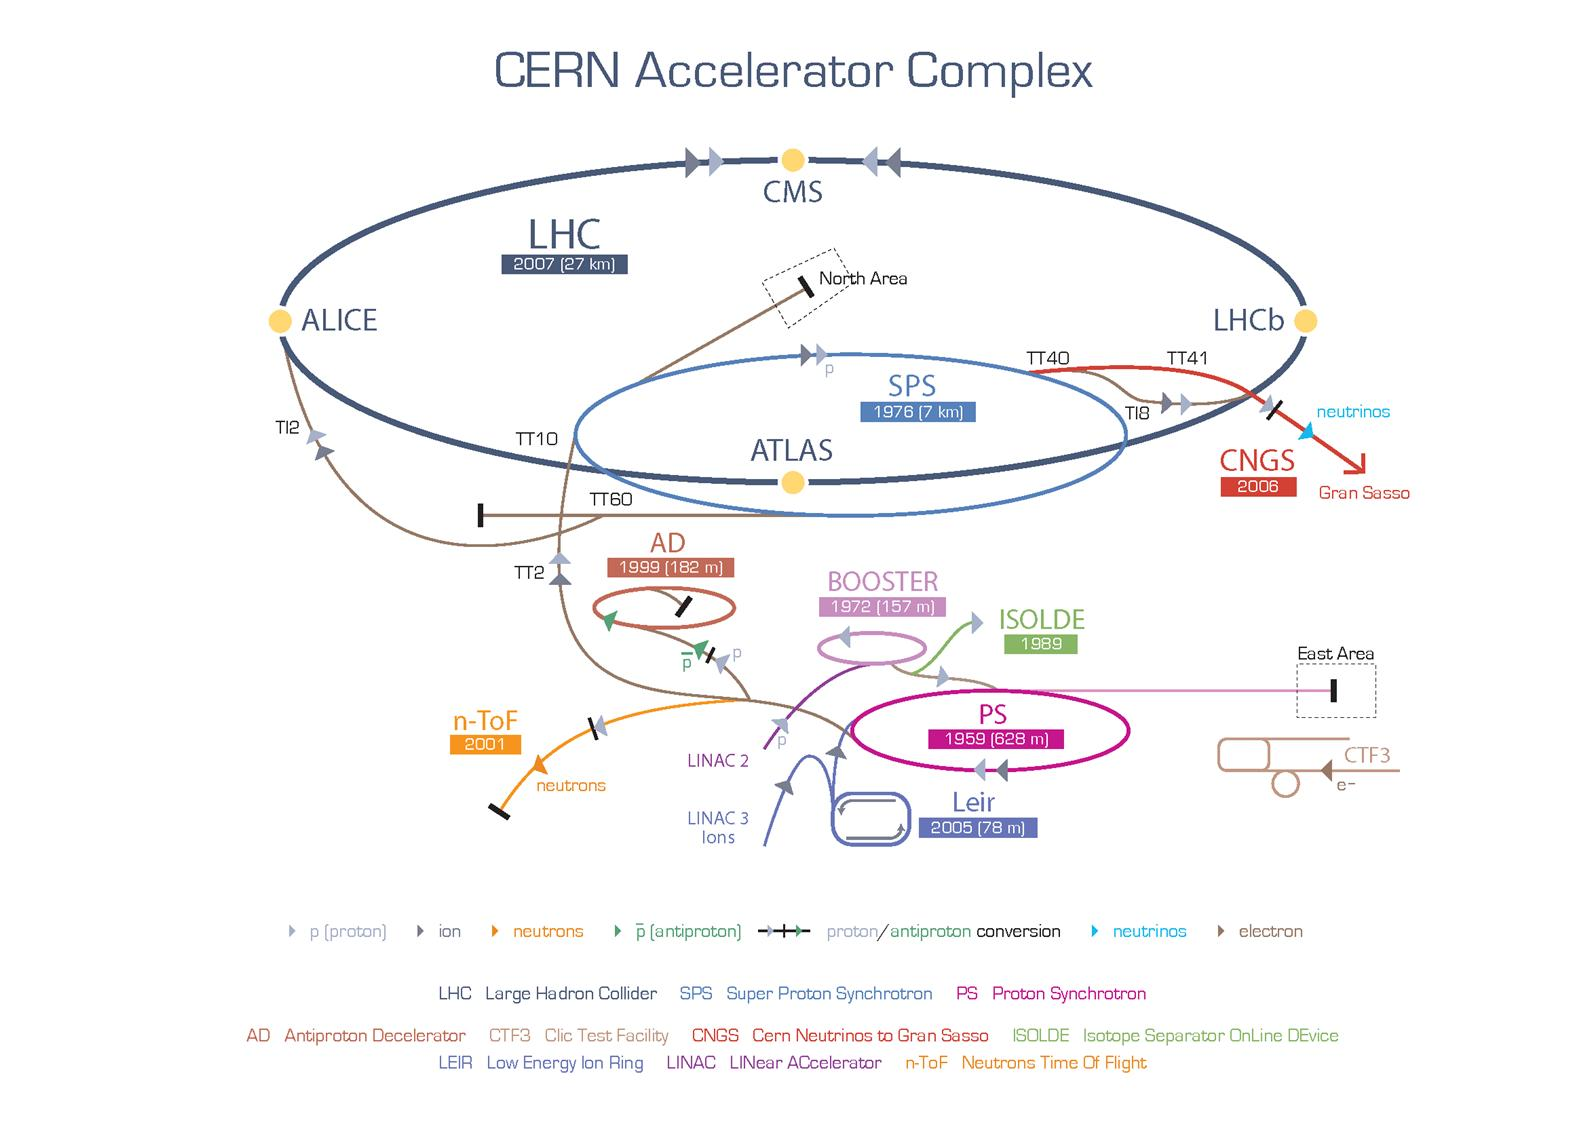
\includegraphics[trim=4.5cm 0cm 0cm 0cm, clip=true, width=1.15\textwidth]{figs/cern-lhc-4.jpg}
    \caption{Organization of CERN complex}
    \label{fig:Complex}
  \end{center}
\end{figure}

\subsection{Injector chain}
\label{sec:injector}

The injector chain begins with the proton source. Protons are extracted via ionization of Hydrogen gas in the Duoplasmatron Proton Ion Source. Such extraction is pulsed, what makes up the first bunch structure. The extracted protons are then accelerated to 50 MeV in the linear accelerator, Linac2, that dates from 1978. After this first stage several steps are followed:
\begin{enumerate}
\item Linac2 injects proton bunches in the Proton Synchrotron Booster (PSB) where are accelerated to 1.4 GeV. 
\item From PSB, the protons are delivered to the Proton Synchrotron (PS) where they reach an energy of 25 GeV. In the PS the bunches are also split from 6 initial bunches to 72 spaced by 25 ns.
\item Finally, the pre-acceleration chain is finished by the SPS, Super Proton Synchrotron. There the bunches are accelerated up to 450 GeV right before being inserted to the main LHC ring. 
\end{enumerate}

The whole pre-acceleration chain has been optimized to obtain the best possible performance on the final acceleration in the LHC main ring. All parameters are carefully controlled, for example the number of bunches, the separation between bunches, the separation between trains of bunches or the injection energy to each subsystem. It's also remarkable to notice the level of control achieved in the bunches manipulation, from old subsystems as the PS from 1959 or the newest, the SPS that dates from 1976. 

Some recent plans for future accelerator have been theorized using the LHC main ring as injector for a bigger accelerator, for example the so called Very Large Hadron Collider or VLHC.  

\subsection{Main ring}
\label{sec:ring}



\section{The Compact Muon Solenoid experiment}
\label{sec:CMS}



\[ f'(x) = 1-2x \]
\[ \beta(x) \leq \cos(x) \]
\[ \sqrt{\frac{1}{2}}=\frac{\sqrt(2)}{2} \]

\begin{equation}
\forall x \in \mathbb{R}, f'(x)=f(x)
\end{equation}

\begin{equation}
\lim_{x\to 0}\frac{\sin(x)}{x}=1
\end{equation}

\begin{equation}
\int_{0}^{\infty}\frac{\ln(x)}{f(x)}=\pi^2
\end{equation}

\begin{equation*}
\left\Vert 2^{\Gamma(x)} \right\Vert^{2} = \underbrace{f(a)+f(b)}_{\leq 1}+\dot{y}
\end{equation*}
